\documentclass[12pt,english,ignorenonframetext,]{beamer}


%%%%%%%%%%%%%%%
%% Beamer theme
% choose one from http://deic.uab.es/~iblanes/beamer_gallery/
% or http://www.hartwork.org/beamer-theme-matrix/
% \usetheme{Warsaw}
\usetheme{CambridgeUS}

%%%%%%%%%%%%%%%%%%%%%%
%% Beamer color theme
%% default albatross beaver beetle crane dolphin dove fly lily
%% orchid rose seagull seahorse whale wolverine

%\usecolortheme{seahorse}  %% very lighty
\usecolortheme{dolphin}    %% nice blue
\usecolortheme{orchid}     %% dark red ?
\usecolortheme{whale}      %% black and blue as Warsaw

%%%%%%%%%%%%%%%%%%%%%%%%%%%%%%%%%%%%%%%%%%%%%%%%%%%%%%%%%%%%%%%%%%%%%%%%%%%%%%%%
%% Define your own colors
\definecolor{blackblue}{rgb}{19,19,59}  % rgb(48,48,150)

%%%%%%%%%%%%%%%%%%%%%%%%%%%%%%%%%%%%%%%%%%%%%%%%%%%%%%%%%%%%%%%%%%%%%%%%%%%%%%%%
%% Change the theme
%\setbeamercolor{alerted text}{fg=orange}
%\setbeamercolor{background canvas}{bg=white}
%\setbeamercolor{block body alerted}{bg=normal text.bg!90!black}
%\setbeamercolor{block body}{bg=normal text.bg!90!black}
%\setbeamercolor{block body example}{bg=normal text.bg!90!black}
%\setbeamercolor{block title alerted}{use={normal text,alerted text},fg=alerted text.fg!75!normal text.fg,bg=normal text.bg!75!black}
%\setbeamercolor{block title}{bg=blue}
%\setbeamercolor{block title example}{use={normal text,example text},fg=example text.fg!75!normal text.fg,bg=normal text.bg!75!black}
%\setbeamercolor{fine separation line}{}
\setbeamercolor{frametitle}{fg=black}
%\setbeamercolor{item projected}{fg=black}
%\setbeamercolor{normal text}{bg=black,fg=yellow}
%\setbeamercolor{palette sidebar primary}{use=normal text,fg=normal text.fg}
%\setbeamercolor{palette sidebar quaternary}{use=structure,fg=structure.fg}
%\setbeamercolor{palette sidebar secondary}{use=structure,fg=structure.fg}
%\setbeamercolor{palette sidebar tertiary}{use=normal text,fg=normal text.fg}
%\setbeamercolor{section in sidebar}{fg=brown}
%\setbeamercolor{section in sidebar shaded}{fg= grey}
\setbeamercolor{separation line}{}
%\setbeamercolor{sidebar}{bg=red}
%\setbeamercolor{sidebar}{parent=palette primary}
%\setbeamercolor{structure}{bg=black, fg=green}
%\setbeamercolor{subsection in sidebar}{fg=brown}
%\setbeamercolor{subsection in sidebar shaded}{fg= grey}
%\setbeamercolor{title}{fg=blackblue}
%\setbeamercolor{titlelike}{fg=blackblue}


%%%%%%%%%%%%%%%%%%%%%%%
%% Other beamer options
%\setbeamercovered{transparent}
% Permet de laisser en gris le texte qui n'est pas encore apparu (lorsqu'on utilise les commandes avec des <1,2> ou <4-9>.

%\setbeamercolor{normal text}{fg=black,bg=white}

%%%%%%%%%%%%%%%%%%%%%%%
%% Change Beamer fonts
% \usefonttheme{default}
% \usefonttheme[onlymath]{serif}
\usefonttheme{serif}

\setbeamerfont{title}{family=\rm}
\setbeamerfont{titlelike}{family=\rm}
\setbeamerfont{frametitle}{family=\rm}

%%%%%%%%%%%%%%%%%%%%%%%%%%%%%%%%%%%%%%%%%%%%%%%%%%%%%%%%%%%%%%%%%%%%%%%%%%%%%%%%
%% innertheme
%% rectangles circles inmargin rounded
% \useinnertheme{rounded}  % XXX My preference
\useinnertheme{circles}    % XXX

%%%%%%%%%%%%%%%%%%%%%%%%%%%%%%%%%%%%%%%%%%%%%%%%%%%%%%%%%%%%%%%%%%%%%%%%%%%%%%%%
%% outertheme
%% infolines miniframes shadow sidebar smoothbars smoothtree split tree
%\useoutertheme{infolines}

%% No navigation symbol.
\setbeamertemplate{navigation symbols}{}
\beamertemplatenavigationsymbolsempty

% XXX Add a background image to the slides
\usepackage{tikz}
% \setbeamertemplate{background}{\includegraphics[width=\paperwidth,height=\paperheight,keepaspectratio]{IETR.jpg}}
% \setbeamertemplate{background}{{\centering\begin{tikzpicture}\node[opacity=0.15]{\includegraphics[width=0.98\paperwidth]{IETR_et_partenaires_IETR.png}};\end{tikzpicture}}}

% Other options
%\setbeamertemplate{footline}[page number]

\beamertemplateballitem
\setbeamertemplate{itemize item}[square]


\setbeamertemplate{caption}[numbered]
\setbeamertemplate{caption label separator}{: }
\setbeamercolor{caption name}{fg=normal text.fg}
\beamertemplatenavigationsymbolsempty
\usepackage{lmodern}
\usepackage{color}
  \newcommand{\urlb}[1]{\textcolor{blue}{\url{#1}}}
%% Color definition
\usepackage{xcolor}
\definecolor{bleu}{RGB}{0,0,204}  % rgb(0,0,204)
\definecolor{violet}{RGB}{102,0,204}  % rgb(102,0,204)
\definecolor{darkgreen}{RGB}{0,100,0}  % rgb(0,100,0)
\definecolor{gold}{RGB}{255,184,0}  % rgb(255,184,0)
\definecolor{rouge}{RGB}{204,0,0}  % rgb(204,0,0)
\usepackage{amssymb,amsmath}
\usepackage{bbm,bm}  % bold maths symbols
\usepackage{ifxetex,ifluatex}
\usepackage{fixltx2e} % provides \textsubscript

\usepackage{macrosText}  % FIXME remove

\ifnum 0\ifxetex 1\fi\ifluatex 1\fi=0 % if pdftex
  \usepackage[T1]{fontenc}
  \usepackage[utf8]{inputenc}
\else % if luatex or xelatex
  \ifxetex
    \usepackage{mathspec}
  \else
    \usepackage{fontspec}
  \fi
  \defaultfontfeatures{Ligatures=TeX,Scale=MatchLowercase}
\fi
% use upquote if available, for straight quotes in verbatim environments
\IfFileExists{upquote.sty}{\usepackage{upquote}}{}
% use microtype if available
\IfFileExists{microtype.sty}{%
\usepackage{microtype}
\UseMicrotypeSet[protrusion]{basicmath} % disable protrusion for tt fonts
}{}
\ifnum 0\ifxetex 1\fi\ifluatex 1\fi=0 % if pdftex
  \usepackage[shorthands=off,main=english]{babel}
\else
  \usepackage{polyglossia}
  \setmainlanguage[]{}
\fi
\newif\ifbibliography
\hypersetup{
            pdftitle={Multi-Player Bandits Models Revisited},
            pdfauthor={  Christophe Moy Émilie Kaufmann},
            pdfborder={0 0 0},
            breaklinks=true}
% \urlstyle{same}  % don't use monospace font for urls
% Code embedding.
\usepackage{palatino}              % Use the Palatino font % XXX remove if it is ugly ?

% Prevent slide breaks in the middle of a paragraph:
\widowpenalties 1 10000
\raggedbottom


\setlength{\parindent}{0pt}
\setlength{\parskip}{6pt plus 2pt minus 1pt}
\setlength{\emergencystretch}{3em}  % prevent overfull lines
\providecommand{\tightlist}{%
  \setlength{\itemsep}{0pt}\setlength{\parskip}{0pt}}
\setcounter{secnumdepth}{5}

% https://tex.stackexchange.com/a/2559/
\newcommand{\backupbegin}{
  \newcounter{framenumberappendix}
  \setcounter{framenumberappendix}{\value{framenumber}}
}
\newcommand{\backupend}{
  \addtocounter{framenumberappendix}{-\value{framenumber}}
  \addtocounter{framenumber}{\value{framenumberappendix}}
}

  \title{Multi-Player Bandits Models Revisited}
  \subtitle{Decentralized Multi-Player Multi-Arm Bandits}
    \author[Lilian Besson]{\textbf{Lilian Besson} \newline \emph{Advised by} \and Christophe Moy
\and Émilie Kaufmann}
        \institute[CentraleSupélec \& Inria]{PhD Student \newline Team SCEE, IETR, CentraleSupélec, Rennes
\newline \& Team SequeL, CRIStAL, Inria, Lille}
        \date[SequeL Seminar - 22/12/17]{SequeL Seminar - 22 December 2017}
  
% For \justifying command, see https://tex.stackexchange.com/a/148696/
\usepackage{ragged2e}
\addtobeamertemplate{frame begin}{}{\justifying}
\addtobeamertemplate{block begin}{}{\justifying}
\addtobeamertemplate{block alerted begin}{}{\justifying}
\addtobeamertemplate{block example begin}{}{\justifying}
\addtobeamertemplate{itemize body begin}{}{\justifying}
\addtobeamertemplate{itemize item}{}{\justifying}
\addtobeamertemplate{itemize subitem}{}{\justifying}
\addtobeamertemplate{itemize subsubitem}{}{\justifying}
\addtobeamertemplate{enumerate body begin}{}{\justifying}
\addtobeamertemplate{enumerate item}{}{\justifying}
\addtobeamertemplate{enumerate subitem}{}{\justifying}
\addtobeamertemplate{enumerate subsubitem}{}{\justifying}
\addtobeamertemplate{description body begin}{}{\justifying}
\addtobeamertemplate{description item}{}{\justifying}

\begin{document}
\justifying

\begin{frame}[plain]
\titlepage

% XXX manual inclusion of logos
\begin{center}
\includegraphics[height=0.16\textheight]{LogoIETR.png}
\includegraphics[height=0.16\textheight]{LogoCS.png}
\includegraphics[height=0.16\textheight]{LogoInria.jpg}
\end{center}

\end{frame}

\section*{\hfill{}CentraleSupélec Rennes \& Inria Lille\hfill{}}

\subsection*{\hfill{}Team {:} SCEE @ IETR \& SequeL @ CRIStAL\hfill{}}




\section{\hfill{}1. Introduction and motivation\hfill{}}

\subsection{\hfill{}1.a. Objective\hfill{}}

\end{frame}

\begin{frame}{Motivation}

A \emph{lot} of communicating devices want to access to a single base
station.

\begin{itemize}
\tightlist
\item
  Insert them in a \textbf{crowded wireless network}.
\item
  With a protocol \textbf{slotted in both time and frequency}.
\end{itemize}

\begin{block}{Goal}

\begin{itemize}
\tightlist
\item
  Maintain a \textbf{good Quality of Service}.
\item
  \textbf{Without centralized supervision} as it costs network overhead.
\end{itemize}

\end{block}

\begin{block}{How?}

\begin{itemize}
\tightlist
\item
  Use \textbf{learning algorithms}: devices will learn on which
  frequency they should talk!
\end{itemize}

\end{block}

\end{frame}



\subsection{\hfill{}1.b. Outline and references\hfill{}}

\end{frame}

\begin{frame}{Outline and references}

\begin{enumerate}
\def\labelenumi{\arabic{enumi}.}
\tightlist
\item
  Introduction and motivation
\item
  Model and hypotheses
\item
  Lower-bound on regret
\item
  Quick reminder on single-player MAB algorithms
\item
  Three new multi-player decentralized algorithms: \MCTopM, \RandTopM,
  \Selfish
\item
  Upper-bound on regret for \MCTopM
\item
  Experimental results
\item
  Disappointing results for \Selfish
\item
  Perspectives and future works
\end{enumerate}

\vfill{}

\begin{footnotesize}
Main references are my recent articles (on HAL):
\begin{itemize}
\item \emph{Multi-Player Bandits Models Revisited}, Besson, Kaufmann. \texttt{arXiv:1711.02317},
\item \emph{Multi-Armed Bandit Learning in IoT Networks and non-stationary settings}, Bonnefoi, Besson, Moy, Kaufmann, Palicot. CrownCom 2017,
\end{itemize}
\end{footnotesize}

\end{frame}



\section{\hfill{}2. Model and hypotheses\hfill{}}

\subsection{\hfill{}2.a. Our model\hfill{}}

\end{frame}

\begin{frame}{Our model}

\begin{itemize}
\tightlist
\item
  Discrete time \(t\geq1\) and \(K\) radio channels (\emph{e.g.}, 10)
  \hfill{} (\emph{known})
\item
  Every time frame:
\end{itemize}

\begin{figure}[h!]
\centering
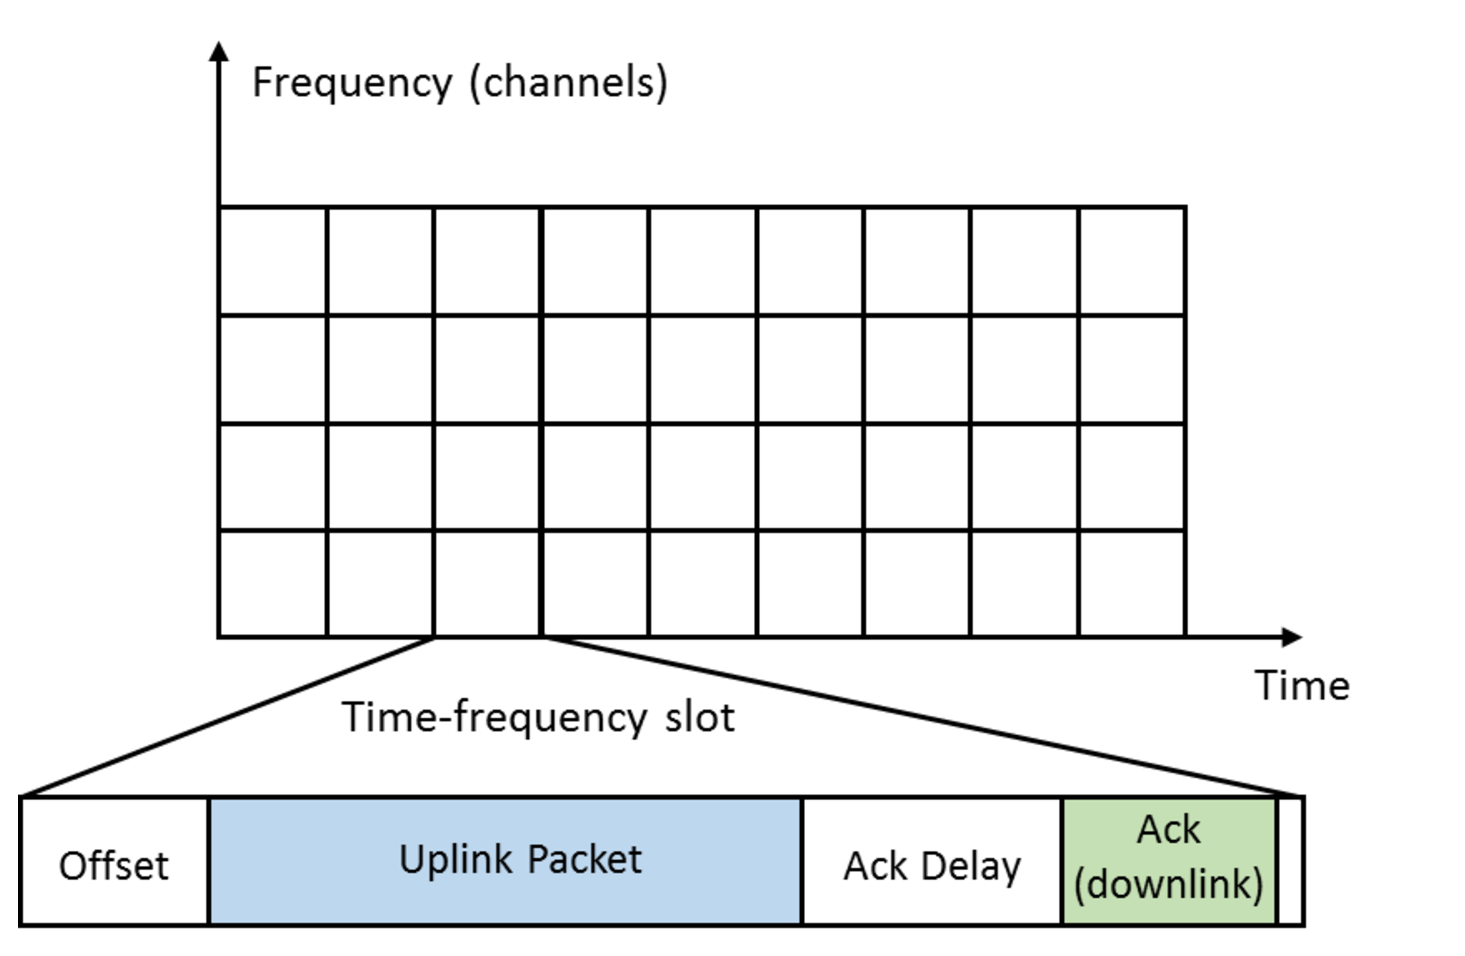
\includegraphics[height=0.35\textheight]{figures/protocol.eps}
\caption{\small{Protocol in time and frequency, with an \textcolor{darkgreen}{\emph{Acknowledgement}}.}}
\end{figure}

\begin{block}{Dynamic radio reconfiguration}

\begin{itemize}
\tightlist
\item
  A \textbf{dynamic device decides the channel it uses to send every
  packet}.
\item
  It has memory and computational capacity to implement simple
  \textbf{decision algorithm}.
\end{itemize}

\end{block}

\end{frame}



\subsection{\hfill{}2.b. With or without sensing\hfill{}}

\end{frame}

\begin{frame}[fragile]{Our model}

\begin{block}{``Easy'' case}

\begin{itemize}
\tightlist
\item
  \(M \leq K\) dynamic devices \textbf{always communicating}, try to
  access the network, \emph{independently}: without any centralized
  supervision!
\item
  Background is \emph{i.i.d.}.
\end{itemize}

\end{block}

\begin{block}{Two variants}

\begin{enumerate}
\def\labelenumi{\arabic{enumi}.}
\item
  \emph{With sensing}: Device first senses for presence of Primary Users
  (background traffic), then use \texttt{Ack} to detect collisions.
  \small{Model the "classical" Opportunistic Spectrum Access problem.
  Not exactly suited for *Internet of Things* networks like LoRa or SigFox, can model ZigBee, and can be analyzed mathematically...}
\item
  \emph{Without sensing}: same background traffic, but cannot sense, so
  \texttt{Ack} is used to know if the message was successfully received
  by the Base Station. (Harder to analyze mathematically.)
\end{enumerate}

\end{block}

\end{frame}



\subsection{\hfill{}2.c. Notations\hfill{}}

\end{frame}

\begin{frame}[fragile]{Notations}

\begin{block}{\emph{i.i.d.} background traffic}

\begin{itemize}
\tightlist
\item
  \(K\) channels, modeled as Bernoulli (\(0/1\)) distributions of mean
  \(\mu_k\) \(=\) background traffic from \emph{Primary Users},
  bothering the dynamic devices!
\item
  \(M\) devices use channel \(A^j(t) \in \{1,\dots,K\}\) at each time
  step,
\end{itemize}

\end{block}

\begin{block}{Rewards}

\begin{itemize}
\tightlist
\item
  Reward:
  \(r^j(t) := Y_{A^j(t),t} \times \mathbbm{1}(\overline{C^j(t)}) = \mathbbm{1}(\)uplink
  \& \texttt{Ack}\()\)

  \begin{itemize}
  \tightlist
  \item
    with sensing information \(Y_{k,t} \sim \mathrm{Bern}(\mu_k)\),
  \item
    collision for device \(j\)
    \(C^j(t) = \mathbbm{1}(\)\emph{alone on arm $A^j(t)$}\()\).
  \end{itemize}
\end{itemize}

\end{block}

\end{frame}



\subsection{\hfill{}2.d. Goal\hfill{}}

\end{frame}

\begin{frame}[fragile]{Goal}

\begin{block}{Problem}

\begin{itemize}
\tightlist
\item
  \emph{Goal} : \emph{minimize packet loss ratio} (\(=\) maximize number
  of received \texttt{Ack}) in a \emph{finite-space discrete-time
  Decision Making Problem}.
\item
  \emph{Solution ?} \textbf{Multi-Armed Bandit algorithms},
  \textbf{decentralized} and used \textbf{independently} by each device.
\end{itemize}

\end{block}

\begin{block}{Goal : \emph{decentralized} reinforcement learning
optimization!}

\begin{itemize}
\tightlist
\item
  Maximize transmission rate \(\equiv\) \textbf{maximize cumulated
  rewards}
  \[\max_{\text{algorithm}\;A} \;\; \sum_{\tau=1}^{\text{horizon}} r_{A(\tau)}.\]
\item
  Each player wants to \textbf{maximize its cumulated reward},
\item
  With no central control, and no exchange of information,
\item
  Only possible if : each player converges to one of the \(M\) best
  arms, orthogonally (without collisions)
\end{itemize}

\end{block}

\end{frame}



\subsection{\hfill{}2.e. Centralized regret\hfill{}}

\end{frame}

\begin{frame}{Centralized regret}

\begin{block}{A measure of success}

\begin{itemize}
\tightlist
\item
  Not the network throughput or collision probability,
\item
  We study the \textbf{centralized regret} \vspace*{-5pt}
  \[ R_T(\boldsymbol{\mu}, M, \rho) := \left(\sum_{k=1}^{M}\mu_k^*\right) T - \E_{\mu}\left[\sum_{t=1}^T\sum_{j=1}^M r^j(t)\right]. \]
\end{itemize}

\pause

\end{block}

\begin{block}{Two directions of analysis}

\begin{itemize}
\tightlist
\item
  Clearly \(R_T = \mathcal{O}(T)\), but we want a sub-linear regret, as
  small as possible!
\item
  \emph{What is the best possible performance of a decentralized
  algorithm in this setting?} \newline
   \hfill{} \(\hookrightarrow\) \textbf{Lower Bound} on regret for
  \textbf{any} algorithm !
\item
  \emph{Is this algorithm efficient in this setting?} \newline
   \hfill{} \(\hookrightarrow\) \textbf{Upper Bound} on regret for
  \textbf{one} algorithm !
\end{itemize}

\end{block}

\end{frame}



\section{\hfill{}3. Lower-bound\hfill{}}

\subsection{\hfill{}3.a. Lower-bound on regret\hfill{}}

\end{frame}

\begin{frame}[allowframebreaks]{Asymptotic Lower Bound on regret}

\begin{block}{Decomposition}

For any algorithm, decentralized or not, we have \vspace*{-20pt}

\begin{small}\begin{align*}
R_T(\boldsymbol{\mu}, M, \rho) &= \sum_{k \in \Mworst} (\mu_M^* -  \mu_k) \E_{\mu}[T_k(T)] \\
&+ \sum_{k \in \Mbest} (\mu_k -  \mu_M^*) (T - \E_{\mu}[T_k(T)]) + \sum_{k=1}^{K} \mu_k \E_{\mu}[\mathcal{C}_k(T)].
\end{align*}\end{small}

\end{block}

\begin{block}{Small regret can be attained if\ldots{}}

\begin{enumerate}
\def\labelenumi{\arabic{enumi}.}
\tightlist
\item
  Devices can quickly identify the bad arms \(\Mworst\), and not play
  them too much (\emph{number of sub-optimal selections}),
\item
  Devices can quickly identify the best arms, and most surely play them
  (\emph{number of optimal non-selections}),
\item
  Devices can use orthogonal channels (\emph{number of collisions}).
\end{enumerate}

\end{block}

\begin{block}{Lower-bounds}

\begin{itemize}
\tightlist
\item
  The first term \(\E_{\mu}[T_k(T)]\), for sub-optimal arms selections,
  is lower-bounded, using technical information theory tools
  (Kullback-Leibler divergence, entropy),
\item
  And we lower-bound the rest (including collisions) by\ldots{} \(0\) :
  we should be able to do better!
\end{itemize}

\end{block}

\begin{block}{Theorem 1
\hfill{}\textcolor{gray}{[Besson \& Kaufmann, 2017]}}

\begin{itemize}
\tightlist
\item
  For any uniformly efficient decentralized policy, and any
  non-degenerated problem \(\boldsymbol{\mu}\), \vspace*{-10pt}
  \[ \mathop{\lim\inf}\limits_{T \to +\infty} \frac{R_T(\boldsymbol{\mu}, M, \rho)}{\log(T)} \geq M \times \left( \sum_{k \in \Mworst} \frac{(\mu_M^* -  \mu_k)}{\kl(\mu_k, \mu_M^*)} \right) . \]
  \footnotetext{\tiny Where $\kl(x,y) := x \log(\frac{x}{y}) + (1 - x) \log(\frac{1-x}{1-y})$ is the binary Kullback-Leibler divergence.}
\end{itemize}

\end{block}

\end{frame}



\subsection{\hfill{}3.b. Illustration of the Lower Bound\hfill{}}

\end{frame}

\begin{frame}[plain]{Illustration of the Lower Bound on regret}

\begin{figure}[h!]
\centering
\includegraphics[height=0.75\textheight]{figures/main_RegretCentralized____env3-4_2092905764868974160.pdf}
\caption{\footnotesize{Any such lower-bound is very asymptotic, usually not satisfied for small horizons. We can see the importance of the collisions!}}
\end{figure}

\end{frame}



\subsection{\hfill{}3.c. Sketch of the proof\hfill{}}

\end{frame}

\begin{frame}[allowframebreaks]{Sketch of the proof}

FIXME

\end{frame}



\section{\hfill{}4. Single-player MAB algorithms : UCB, KL-UCB, TS\hfill{}}

\subsection{\hfill{}4.a. Upper Confidence Bound algorithm : UCB\hfill{}}

\end{frame}

\begin{frame}{Upper Confidence Bound algorithm (\(\mathrm{UCB}_1\))}

Dynamic device keep \(\tau\) number of sent packets, \(T_k(\tau)\)
selections of channel \(k\), \(X_k(\tau)\) successful transmission in
channel \(k\).

\begin{enumerate}
\def\labelenumi{\arabic{enumi}.}
\tightlist
\item
  For the first \(K\) steps (\(\tau=1,\dots,K\)), try each channel
  \emph{once}.
\item
  Then for the next steps \(t > K\) :

  \begin{itemize}
  \tightlist
  \item
    Compute the index
    \(g_k(\tau) := \underbrace{\frac{X_k(\tau)}{T_k(\tau)}}_{\text{Mean}\; \widehat{\mu_k}(\tau)} + \underbrace{\sqrt{\frac{\log(\tau)}{2 T_k(\tau)}},}_{\text{Upper Confidence Bound}}\)
  \item
    Choose channel
    \(A(\tau) = \mathop{\arg\max}\limits_{k} \; g_k(\tau)\),
  \item
    Update \(T_k(\tau+1)\) and \(X_k(\tau+1)\).
  \end{itemize}
\end{enumerate}

\vfill{}\hfill{}\tiny{\textcolor{gray}{References: [Lai \& Robbins, 1985], [Auer et al, 2002], [Bubeck \& Cesa-Bianchi, 2012]}}

\end{frame}



\subsection{\hfill{}4.b. Kullback-Leibler UCB algorithm : KL-UCB\hfill{}}

FIXME update

\end{frame}

\begin{frame}{Kullback-Leibler UCB algorithm
(\(\mathrm{KL}\)-\(\mathrm{UCB}\))}

Dynamic device keep \(\tau\) number of sent packets, \(T_k(\tau)\)
selections of channel \(k\), \(X_k(\tau)\) successful transmission in
channel \(k\).

\begin{enumerate}
\def\labelenumi{\arabic{enumi}.}
\tightlist
\item
  For the first \(K\) steps (\(\tau=1,\dots,K\)), try each channel
  \emph{once}.
\item
  Then for the next steps \(t > K\) :

  \begin{itemize}
  \tightlist
  \item
    Compute the index
    \(g_k(\tau) := \underbrace{\frac{X_k(\tau)}{T_k(\tau)}}_{\text{Mean}\; \widehat{\mu_k}(\tau)} + \underbrace{\sqrt{\frac{\log(\tau)}{2 T_k(\tau)}},}_{\text{Upper Confidence Bound}}\)
  \item
    Choose channel
    \(A(\tau) = \mathop{\arg\max}\limits_{k} \; g_k(\tau)\),
  \item
    Update \(T_k(\tau+1)\) and \(X_k(\tau+1)\).
  \end{itemize}
\end{enumerate}

\vfill{}\hfill{}\tiny{\textcolor{gray}{References: [Lai \& Robbins, 1985], [Auer et al, 2002], [Bubeck \& Cesa-Bianchi, 2012]}}

\end{frame}



\subsection{\hfill{}4.c. Thompson Sampling : Bayesian index policy\hfill{}}

FIXME remove this

\end{frame}

\begin{frame}[fragile]{Thompson Sampling : Bayesian approach}

A dynamic device assumes a stochastic hypothesis on the background
traffic, modeled as Bernoulli distributions.

\begin{itemize}
\item
  Rewards \(r_k(\tau)\) are assumed to be \emph{i.i.d.} samples from a
  Bernoulli distribution \(\mathrm{Bern}(\mu_k)\).
\item
  A \textbf{binomial Bayesian posterior} is kept on the mean
  availability \(\mu_k\) :
  \(\mathrm{Bin}(1 + X_k(\tau), 1 + T_k(\tau) - X_k(\tau))\).
\item
  Starts with a \emph{uniform prior} :
  \(\mathrm{Bin}(1, 1) \sim \mathcal{U}([0,1])\).
\end{itemize}

\begin{enumerate}
\def\labelenumi{\arabic{enumi}.}
\tightlist
\item
  Each step \(\tau \geq 1\), draw a sample from each posterior
  \(i_k(\tau) \sim \mathrm{Bin}(a_k(\tau), b_k(\tau))\),
\item
  Choose channel \(A(\tau) = \mathop{\arg\max}\limits_k \; i_k(\tau)\),
\item
  Update the posterior after receiving \texttt{Ack} or if collision.
\end{enumerate}

\vfill{}\hfill{}\tiny{\textcolor{gray}{References: [Thompson, 1933], [Kaufmann et al, 2012]}}

\end{frame}



\section{\hfill{}5. Multi-player decentralized algorithms: \MCTopM, \RandTopM, \Selfish{} \hfill{}}\subsection{\hfill{}5.a. State-of-the-art MP algorithms\hfill{}}

\end{frame}

\begin{frame}{Algorithms for this easier model}

\begin{block}{Building blocks : separate the two aspects}

\begin{enumerate}
\def\labelenumi{\arabic{enumi}.}
\tightlist
\item
  \textbf{MAB policy} to learn the best arms (use sensing
  \(Y_{A^j(t),t}\)),
\item
  \textbf{Orthogonalization scheme} to avoid collisions (use
  \(C^j(t)\)).
\end{enumerate}

\pause

\end{block}

\begin{block}{Many different proposals for \emph{decentralized} learning
policies}

\begin{itemize}
\tightlist
\item
  Recent: \MEGA{} and \MusicalChair{},
  \hfill{}{\tiny \textcolor{gray}{[Avner \& Mannor, 2015], [Shamir et al, 2016]}}
\item
  State-of-the-art: \textbf{RhoRand policy} and variants,
  \hfill{}{\tiny \textcolor{gray}{[Anandkumar et al, 2011]}}
\item
  \textbf{Our proposals}:
  \hfill{}{\tiny \textcolor{gray}{[Besson \& Kaufmann, 2017]}}

  \begin{itemize}
  \tightlist
  \item
    With sensing: \RandTopM{} and \MCTopM{} are sort of mixes between
    RhoRand and \MusicalChair{}, using UCB indexes or more efficient
    index policy (\klUCB),
  \item
    Without sensing: \Selfish{} use a UCB index directly on the reward
    \(r^j(t)\) : like the first IoT model !
  \end{itemize}
\end{itemize}

\end{block}

\end{frame}



\subsection{\hfill{}5.b. \RandTopM{} algorithm\hfill{}}

\end{frame}

\begin{frame}{The \RandTopM{} algorithm}

FIXME include code, explain

\end{frame}



\subsection{\hfill{}5.c. \MCTopM{} algorithm\hfill{}}

\end{frame}

\begin{frame}{The \MCTopM{} algorithm}

FIXME include code, explain FIXME include figure, explain

\end{frame}



\section{\hfill{}6. Regret upper-bound\hfill{}}\subsection{\hfill{}6.a. \MCTopM-\klUCB\hfill{}}

\end{frame}

\begin{frame}{Regret upper-bound for \MCTopM-\klUCB}

\begin{block}{Theorem 2
\hfill{}\textcolor{gray}{[Besson \& Kaufmann, 2017]}}

\begin{itemize}
\tightlist
\item
  If all \(M\) players use \MCTopM-\klUCB, then for any non-degenerated
  problem \(\boldsymbol{\mu}\), there exists a problem dependent
  constant \(G_{M,\boldsymbol{\mu}}\) , such that the regret satisfies:
  \[
    R_T(\boldsymbol{\mu}, M, \rho) \leq G_{M,\boldsymbol{\mu}} \log(T) + \smallO{\log T}.
  \]
\end{itemize}

\end{block}

\begin{block}{Remarks}

\begin{itemize}
\tightlist
\item
  Hard to prove, we had to carefully design the \MCTopM{} algorithm to
  conclude the proof, 
\item
  For the suboptimal selections, we \emph{match our lower-bound} !
\item
  We also \emph{minimize the number of channel switching}: interesting
  as it costs energy,
\item
  Not yet possible to know what is the best possible control of
  collisions\ldots{}
\end{itemize}

\end{block}

\end{frame}



\subsection{\hfill{}6.b. Sketch of the proof\hfill{}}

\end{frame}

\begin{frame}[allowframebreaks]{Sketch of the proof}

FIXME

\end{frame}



\section{\hfill{}7. Experimental results\hfill{}}\subsection{\hfill{}7.a. Illustration of regret\hfill{}}

\end{frame}

\begin{frame}[plain]{Illustration of regret of different algorithms}

\begin{figure}[h!]
\centering
\includegraphics[height=0.75\textheight]{figures/MP__K9_M6_T5000_N500__4_algos/all_RegretCentralized____env1-1_8318947830261751207.pdf}
\caption{\footnotesize{Regret, $M=6$ players, $K=9$ arms, horizon $T=5000$, against $500$ problems $\boldsymbol{\mu}$ uniformly sampled in $[0,1]^K$. \newline \textcolor{blue}{\rhoRand{}} < \textcolor{red}{\RandTopM{}} < \textcolor{darkgreen}{\Selfish{}} < \textcolor{gold}{\MCTopM{}} in most cases.}}
\end{figure}

FIXME include graph!

\subsection{\hfill{}7.b. Best arm selection\hfill{}}

\end{frame}

\begin{frame}[plain]{Best arm selection}

FIXME include graph!

\subsection{\hfill{}7.c. Number of collisions\hfill{}}

\end{frame}

\begin{frame}[plain]{Number of collisions}

FIXME include graph!

\subsection{\hfill{}7.d. Number of arm switches\hfill{}}

\end{frame}

\begin{frame}[plain]{Number of arm switches}

FIXME include graph!

\subsection{\hfill{}7.e. Fairness\hfill{}}

\end{frame}

\begin{frame}[plain]{Fairness}

FIXME include graph!

\end{frame}



\section{\hfill{}8. Disappointing results for \Selfish\hfill{}}\subsection{\hfill{}8.a. Problems with \Selfish\hfill{}}

FIXME

\end{frame}

\begin{frame}{In this model}

The \Selfish{} decentralized approach = device don't use sensing, just
learn on the receive acknowledgement,

\begin{itemize}
\tightlist
\item
  More suited to model IoT networks,
\item
  Use less information, and don't know the value of \(M\): we expect
  \Selfish{} to not have stronger guarantees.
\item
  It works fine in practice!
\item
  Except\ldots{} when it fails drastically!
\item
  In small problems with \(M\) and \(K = 2\) or \(3\), we found small
  probability of failures (\emph{i.e.}, linear regret), and this
  prevents from having a generic upper-bound on regret for \Selfish.
  Sadly\ldots{}
\end{itemize}

\end{frame}



\subsection{\hfill{}8.b. Failing cases for \Selfish\hfill{}}

\end{frame}

\begin{frame}[plain]{Illustration of failing cases for
\(\mathrm{Selfish}\)}

\begin{figure}[h!]
\centering
\includegraphics[height=0.60\textheight]{figures/MP__K3_M2_T5000_N1000__4_algos/all_HistogramsRegret____env1-1_5016720151160452442.pdf}
\caption{\footnotesize{Regret for $M=2$ players, $K=3$ arms, horizon $T=5000$, $1000$ repetitions and $\boldsymbol{\mu} = [0.1, 0.5, 0.9]$. Axis $x$ is for regret (different scale for each), and \textcolor{darkgreen}{\Selfish{}} have a small probability of failure ($17$ cases of $R_T \geq T$, out of $1000$). The regret for the three other algorithms is very small for this ``easy'' problem.}}
\end{figure}

\end{frame}



\section{\hfill{}9. Perspectives and future work\hfill{}}\subsection{\hfill{}9.a. Perspectives\hfill{}}

\end{frame}

\begin{frame}{Perspectives}

\begin{block}{Theoretical results}

\begin{itemize}
\tightlist
\item
  MAB algorithms have guarantees for \emph{i.i.d. settings},
\item
  But here the collisions cancel the \emph{i.i.d.} hypothesis,
\item
  Not easy to obtain guarantees in this mixed setting \newline
   (\emph{i.i.d.} emissions process, ``game theoretic'' collisions).
\item
  For OSA devices (always emitting), we obtained strong theoretical
  results,
\item
  But harder for IoT devices with low duty-cycle\ldots{}
\end{itemize}

\end{block}

\begin{block}{Real-world experimental validation ?}

\begin{itemize}
\tightlist
\item
  Radio experiments will help to validate this.
  \hspace*{40pt}\hfill{}\textcolor{red}{Hard !}
\end{itemize}

\end{block}

\end{frame}



\subsection{\hfill{}9.b. Future work\hfill{}}

\end{frame}

\begin{frame}{Other directions of future work}

\begin{itemize}
\item
  \emph{More realistic emission model}: maybe driven by number of
  packets in a whole day, instead of emission probability.
\item
  Validate this on a \emph{larger experimental scale}.
\item
  Extend the theoretical analysis to the large-scale IoT model, first
  with sensing (\emph{e.g.}, models ZigBee networks), then without
  sensing (\emph{e.g.}, LoRaWAN networks).
\item
  And also conclude the Multi-Player OSA analysis (remove hypothesis
  that objects know \(M\), allow arrival/departure of objects,
  non-stationarity of background traffic etc)
\end{itemize}

\end{frame}



\section{\hfill{}9. Conclusion\hfill{}}\subsection{\hfill{}9.c. Thanks!\hfill{}}

\end{frame}

\begin{frame}[allowframebreaks]{Conclusion}

\begin{block}{We showed}

\begin{itemize}
\tightlist
\item
  Simple Multi-Armed Bandit algorithms, used in a Selfish approach by
  IoT devices in a crowded network, help to quickly learn the best
  possible repartition of dynamic devices in a fully decentralized and
  automatic way,
\item
  For devices with sensing, smarter algorithms can be designed, and
  analyze carefully.
\item
  Empirically, even if the collisions break the \emph{i.i.d} hypothesis,
  stationary MAB algorithms (UCB, TS, \klUCB) outperform more generic
  algorithms (adversarial, like Exp3).
\end{itemize}

\end{block}

\begin{block}{But more work is still needed\ldots{}}

\begin{itemize}
\tightlist
\item
  \textbf{Theoretical guarantees} are still missing for the IoT model,
  and can be improved (slightly) for the OSA model.
\item
  Maybe study \textbf{other emission models}.
\item
  Implement and test this on \textbf{real-world radio devices} (almost
  done).
\end{itemize}

\end{block}

\begin{block}{\textbf{Thanks!}}

\begin{center}\begin{Large}
\emph{Any question?}
\end{Large}\end{center}

\end{block}

\end{frame}

\end{document}
